% SPDX-License-Identifier: Apache-2.0
% Copyright (c) Contributors to the PhysLight Project.

\chapter{Introduction}


\ifomit


color responsivity in XYZ or in camera RGB?
exposure vs density curve plots




test: try the siggraph font styles
test: try Libertine for body text

\fi

\section{Physical units and digital image synthesis}
%
\epigraph{%
	\emph{Pictures shall be based on models built from Euclidean geometry
		in three dimensions, viewed in two dimensions with Reinassance perspective
		and use Newtonian physics. [...] 
		there is nothing about computers or computation that forces these choices}}
		{\textsc{Alvy Ray Smith}, \emph{The Central Dogma}}

\noindent One of the reasons physically-based image synthesis has become such an
indispensable ingredient for pushing realism and consistency in very
complex scenarios is predictability. 
In fact it is generally assumed that what is needed is an image synthesis system
capable of \emph{photorealism}, that is a system that \emph{given the virtual 
	description of a scene consisting of geometry, material, light sources and cameras
	produce a photorealistic image of it, as if it were captured by a real camera.
	This problem is known as light transport simulation}\footnote{
	This specific phrasing is due to Alexander Rath, during the technical talk at 
	Siggraph 2023 presenting~\cite{rath23}}.


Material modelling is based on physical properties and thus allows to reproduce 
increasingly complex natural phenomena. 
In traditional rendering systems, before the advent of physically-based light transport, 
control of the look of a material was generally owned by the \gls{shading system}.
The \glspl{shader} would be essentially arbitrary pieces of code in charge of computing
the color of an object at a location requested by the renderer. 
Their programmable nature was used for essentially three purposes:
the first was to compute an object's appearance, for example accessing \emph{texture maps},
the second was to compute how light would interact with the material being modeled, often including
all sorts of approximations to overcome shortcomings in the renderer available at the time 
(for example, missing support for indirect illumination),
the third was to \emph{overdrive} the appearance, taking it beyond what would have been possible in a real-life
counterpart, to achieve various kinds of artistic effects.

The physically-based rendering paradigm dictates that \glspl{material model},
lighting and camera response are independent entities and
must hence always be controlled with this separation in mind. 
This makes \gls{virtual} assets more reusable, 
and allows to achieve better consistency when integrating 
digitally produced content with live action \gls{footage}.
This also reduces the scope of the shaders, that end up losing the ability
to \emph{overdrive} and remain more connected to a physically-correct 
model of the world.

Naturally, since a wide range of different effects interplay with each
other in complex and subtle ways, it is absolutely crucial that all
components are accurately represented by their virtual analogues to be
able to reproduce real-world footage realistically. 
Furthermore, the description of the \gls{virtual scene} being based on
real-world quantities enables easier control and verification.




In this document we focus on the specification of \gls{virtual} \glspl{illuminant} and
\glspl{sensor} and make the case for using the same conventions and physical units as
used by lighters and photographers on a motion picture set or in a photographic studio. 
For example, it is preferable in terms of predictability to think about brightness of a 
light source in terms of \glsdisp{photometry}{photometric} units, i.e., units which represent brightness as
perceived by a \gls{human observer}, rather than \glsdisp{radiometry}{radiometric} ones 
(commonly called \gls{wattage}) for two reasons: 
firstly there is convention: the normally used wattage reported on a light fixture or bulb 
is a measure of the power absorbed by the object, not the power of the radiation it emits 
\emph{in the visible range}\footnote{This is effectively the concept of  
	\textsl{\gls{luminous efficacy}}, being the ratio of power absorbed by the emitter
	to the luminous power emitted. 
	What used to be the common household lightbulb, containing incandescent tungsten and 
	rated for 100W, had a luminous efficacy of roughly $15\unit{\lumen\per\watt}$, 
	a contemporary \glsname{LED} lightbulb would be somewhere between 
	$100\unit{\lumen\per\watt}$ and $200\unit{\lumen\per\watt}$, 
	a Xenon arc-lamp somewhere between $30\unit{\lumen\per\watt}$ and
	$90\unit{\lumen\per\watt}$. 
	Note that conservation of energy dictates that when considering all the
	radiation emitted by the bulb, the total radiated power \emph{must} be equal 
	to the absorbed ``electrical'' power} onto the \gls{scene}. 
Secondly, the perceived \gls{brightness} of a source has a fairly marked dependence on 
its color, making lights emitting the same amount of radiative power (even when measured 
limited to the visible spectrum only) appear to have different brightnesses. 

We want instead to specify a system of units and models, in such a manner that
given a real-world scene and a virtual model of it,
specifying the same illuminants via our chosen units, using the same
camera settings and feeding the scene to a compliant renderer will replicate 
the same pixel values as would come from a real-world camera places in the 
real-world version. 
Naturally, for reproducing color, we will not only need
to develop an accurate understanding of brightness, but also be aware
of how \gls{spectral} data flows through the \gls{pipeline}.



The resulting system has been in use in the
production pipeline at \companyname{W\=et\=a FX} since about 2015.
Because of the origin of this system in the motion picture industry,
several terms of the trade have made it into this document. 


The prevalent way of reasoning about image synthesis through rendering is 
built on the notion of the \textsl{light ray}, which is the fundamental element 
of geometrical optics. 
Light rays are the path segments\footnote{
	In the vast majority of renderers in use today, rays are implemented as 
	straight line segments, which enormously simplifies the implementation of the
	code that finds their endpoints. This ignores two effects: the first is that 
	gravity bends light rays and the second it that variations in the index
	of refraction will alter the direction of a light ray.
	Usually bending resulting from gravity won't be an important effect except 
	for scenes that are particularly large and include body with very high mass 
	concentrations like black holes.
	Scenes like this are occasionally rendered, though: for example the 
	movie~\cite{interstellar2014} did need to capture the bending effect of 
	gravity onto light paths accurately, and a specialized rendering system 
	was developed for use on the show. 
	The task was complex enough that the Nobel laureate and CalTech professor 
	Kip Thorne was included as consultant to support the team developing this 
	technology. 
	The second effect ignored by the straight-line approximation is that 
	variations in the index of refraction will also bend the light paths. 
	This is a substantially more common effect at human scale, for example 
	it's the origin of the \textsl{mirage} phenomenon. 
	While there are several research projects that have built renderers able 
	to capture this effect, the computational costs associated with this capability 
	are high enough to make it impractical for everyday use, a recent example
	of this kind of work was described in~\cite{fraboni23}.
	Renderers and transport models built on the \emph{wave optics} model also exist,
	a recent example being described in~\cite{yu23}
} through space that light follows when traveling across the \gls{virtual scene}. 

This document is divided in parts: \cref{part:models}
contains an introduction on basic quantities that are relevant in
light transport simulation and review the relation of photometric and
radiometric units and describes the modelling aspects. In 
\cref{ch:lighting} we describe imaging and light models and propose the
relevant sets of parameters to specify them accurately.  
\Cref{ch:calcsheets} provides some examples on how to derive some of
the described quantities from real world examples.

\Cref{part:ref} provides a reference covering measurements of various 
illuminants (\cref{ch:illuminants}) and cameras (\cref{ch:sensors}).

\Cref{part:app} contains the appendices: \cref{ch:color} discusses
various considerations on color, in particular covering the relation between 
the tristimulus versus spectral settings,
\cref{ch:implementation} describes an implementation of a color manipulation library
and \cref{ch:radiance} is an extensive excerpt from Frederic Nicodemus's 
excellent 1963 paper~\cite{nicodemus63} in which the concept of \textsl{\gls{radiance}}
is introduced: unsurprisingly we found his explanation far clearer than what we 
had been able to come up with, so we decided to retype his words, with the only change being
we have changed the equations to use current conventions for quantity names and symbols, 
and adopted \glsname{si} units throughout.

Because this document is the result of work started from the movie industry, 
we are aware several concepts may not be as well known to our readers from different backgrounds. 
For this reasons we have compiled a reference of notation and symbols used in~\cref{ch:notation} 
as well as a glossary in \cref{sec:main} with the hope these might help clarify potential issues arising 
from our use of movie-making jargon.

\section{Quantities in light transport}
\epigraph{%
	\emph{It has been	my experience that most people find it peculiarly difficult to master 
	the fundamental concepts and relations of radiometry (or photometry) as they apply 
	to extended sources. And I have come to believe that the key to this difficulty 
	lies in the interrelated concepts of an elementary beam of radiation and its 
	radiance (or luminance)}}{\textsc{Fred Nicodemus}, 1963}

\noindent We discussed how \gls{rendering} is concerned with simulating how light travels around in 
a \gls{virtual scene}, so this section introduces names for the quantities transported 
along these paths during the simulation and outlines the theory behind them. 
The naming we adopt was originally introduced by Fred Nicodemus in~\cite{nicodemus77} and
is in line with several current international standards,  
among which we mention \gls{ISO}/\gls{IEC} Standard 80000, 
\emph{Quantities and units, part 7: Light and radiation}~\cite{iso:80000-7:2019}, 
the \emph{International lighting vocabulary} published\footnote{Can also be consulted 
	online at \url{https://cie.co.at/e-ilv}} by the \gls{CIE}~\cite{cie:s017.2020},
and the lighting section of the so-called ``Electropedia'' from the \gls{IEC}~\cite{iec:60050-845:2020}.
Work in recent years has gone into harmonizing these bodies of knowledge so that the resulting 
vocabularies and symbols are in alignment. All the units in use descend directly
from the \gls{si}, descibed in~\cite{bipm:si.2019}.

Thinking about light flowing through a scene, rendering is concerned with the so-called
\textsl{particle theory} of light: these particles are called \textsl{photons}, 
and \textsl{light rays} represent paths along which these photons flow.
The particle theory of light describes a photon as a very small ``object'' 
(a \textsl{particle}) having no mass and no electrical charge, 
instead being made entirely of energy\footnote{
	All readers troubled by this description are in good company. In fact there are 
	certainly substantial theoretical and experimental problems in describing precisely
 	aspects of a photon-as-particle such as its position. 
 	This is an instance of \textsl{Heisenberg uncertainty}
 	and it only begins to scratch the surface of the problems in this area}. 
Max Planck talked about energy \textsl{quanta}: because of what photons are 
(namely, little ``drops'' of energy), 
energy can only come to be in certain specific amounts as can be captured by integral 
amounts of photons. There is no such thing as $1.736$ photons: because photons are integer and 
indivisible, they are viewed in this theory as \textsl{elementary particles}, 
so one can only have 1 photon, or 2 photons or 3 and so on, and this limits the possible
amounts of energy one can have.

As each photon effectively \emph{is} a (small) quantity of energy, there comes about the natural
question of how much energy a given photon actually is. 
It turns out that this depends on the photon's \textsl{\gls{wavelength}} $\lambda$ and is equal 
to $Q_p = hc/\lambda$, where $h$ is a universal constant named after Planck himself
and $c$ is the speed of light in vacuum\footnote{This concept of \textsl{wavelength} hints 
	at the other way of thinking about light, the so-called \textsl{wave theory} of light. 
	The wave theory says that light exists in a \textsl{field} that is 
	present everywhere along our ``light ray'' and is called \textsl{wave} because the strength 
	of this field oscillates over time at a given frequency $\nu = c/\lambda$, 
	measured in $[\unit\hertz]$. 
	In fact, the energy of a photon is technically defined as $Q_p = h\nu$. 
	Because we're mainly concerned with a geometric-optics/particle-theory view of light, 
	in this work we have chosen to work with wavelengths, so we won't
	see much discussion, if any, of frequency and $\nu$'s}. 
The subscript $\square_p$ indicates we are discussing photon quantities: 
we will need to introduce more of these subscripts as we go along to differentiate under 
what perspective we are considering the quantities in play.
For what concerns graphics and rendering, light rays are \textsl{thin} objects, by which we mean 
if we imagined a ray like a tube, or a pipe, it would have a cross section, or width, of $0$. 
However it is occasionally useful to think about the ``size'' of a photon, and it turns out a 
good model for a photon's size is to use its wavelength as a measure of its cross-section diameter.
This is far from an abstract concern: photons will only travel through openings that are bigger 
than their own size (which is relatively natural to expect, thinking about photons as particles).
They will also be relatively undisturbed by things that are substantially smaller than their
size (which instead is natural to expect from a view where photons are waves: it's similar to
how you would observe waves in a lake behave).

As much as photons are the elemental ingredients of light transport, 
they obviously must come from somewhere, which we call \textsl{light sources}.
Given a light source that has been shining for a period of time, it will have emitted a
certain number $N_p$ of photons, delivering a corresponding amount of energy $Q_e$, measured in
joule $[\unit{\joule}]$. Note how the subscript here is $\square_e$, for \textsl{energetic}, indicating
we are looking at a quantity coming from \textsl{\gls{radiometry}}. 
If all of these photons had the same wavelength $\lambda$, maybe because they were coming 
from a laser source, we would have $Q_e = N_p Q_p = N_p  hc/\lambda$. In the general case
of light sources emitting in several different frequencies, we'd have to tally them separately
and sum patiently, or integrate their distribution if we had access to it.

One way or the other, this brings us to discuss the notion of \textsl{power} of our source, 
being its ability to emit light over time. 
Given that light is energy, and as we said we measure energy in $[\unit\joule]$, the emission 
rate of light (which \emph{is} energy) over time $Q_e/t$ will be measured in 
watts $[\unit\watt]$, being joules per second $[\unit\watt] = [\unit{\joule\per\second}]$. 
This under the assumption that our source emits light at a constant rate, and indeed
one might as well think of it as $N_p$ photons per second, as long as one also tallies
accurately the various wavelenghts of these emitted photons exiting the source.
We will come back to this point later in this work, because it's the key ingredient to be able to
discuss the light's \emph{\gls{color}}, which is of course a matter of central importance in
our discussion.

What we are going to do over the rest of this section is to continue to break down 
this aggregate notion of ``energy from a light source'' into simpler components, aiming 
to understand what quantity flows through one ``ray of light'' in more of a ``bulk'' way,
and we'll eventually double back and reason about the color of this light.
For this reason, we were saying we had received from a light source $S$, a certain amount
of energy $Q_e\;[\unit\joule]$. 
If we got this energy over a certain period of time 
$t\;[\unit\second]$ (measured in seconds) at a constant rate, 
we can determine the light's power as $\Phi_e = Q_e / t\;[\unit\watt]$.
Due to the fact that it is said that such a source \textsl{radiates} energy, this quantity
$\Phi_e$ is called the \textsl{radiant power} of the source. 
Further, because it's a measure of how much energy \textsl{flows} out of it, it is also equivalently
called the source's \textsl{radiant flux}, which is why the symbol is $\Phi$, 
the greek letter for sound `f'.

This idea of flow makes it relatively natural to think about light flowing \emph{through}
something like a window, a door, more technically called an \textsl{\gls{aperture}}. 
Obviously light can flow into an aperture just as well as it can flow out of it:
when light leaves an aperture we will say that the quantity is \textsl{\gls{exitant}},
for example we could talk of ``exitant radiant power'' to indicate light leaving from an
aperture flowing out of it, whereas when light arrives at an aperture flowing into it 
we will say it is \textsl{\gls{incident}} to it. 
Lastly, as much as it's valuable to discuss light through a specific given aperture,
sometime we will want to talk about all the light that leaves a source without much of an
interest as to where exactly this flow happens: in this case the mental model
is to think about all light flowing through an imaginary sphere surrounding the whole source.
When there is a need to underline that we're talking about all the light in this sense, we will use the
adjective \textsl{total}, so for a light source we will say in short ``radiant power'' in
most cases meaning ``total exitant radiant power''.

This sphere idea is the key to understand the so-called \textsl{inverse square law}
for light intensity: we will see in a moment that our everyday sense of a light's brightness
is how much energy we receive at a location of interest in terms of its density over area.
In the simple case where the light emits photons uniformly in all directions, the area density
of their flow at a distance $r\;[\unit\meter]$ from their origin will be $\Phi_e / (4\pi r^2)$ 
(being total power for the source divided by the surface area of the sphere). 
You can see that if you grow the area of the sphere this area density will go down 
like the square of the radius, being the distance from the source, 
while conservation of energy will keep the light's power $\Phi_e$ unchanged.

It is natural to think of radiant power as originating from a location $x$ on our source,
or more formally we should say a small region $\delta S$ around $x$ on the source:
for instance a source like a stained glass window would transmit different amounts of energy 
across its surface, as a consequence of the different absorptions of the various pieces of
colored glass that it's made of. 
This leads to an intuitive notion of radiant power from a specific point $x$ on the surface 
of the source $M_e(x)$, and we would like this to be defined so that total power 
from the source $S$ would be computed directly by integration over all of its surface $S$:
\begin{displaymath}
	\Phi_e = \int_{S} M_e(x) \d x \qquad [\unit{\watt}]
\end{displaymath}
this quantity $M_e$ is called \textsl{radiant exitance} and represents the area density
of radiant power emitted by a source, formally
\begin{displaymath}
	M_e = \frac{\d\Phi_e}{\d S} \qquad \left[\unit{\watt\per\square\meter}\right]
\end{displaymath}
In the simple case where we have a uniformly emissive source the
radiant exitance is simply the ratio of emissive power to its area
$M_e = \Phi_e / S$.

Note that this concept of exitance only covers the direct \textsl{\gls{emission}} from a surface,
typical case being its emission as a \textsl{\gls{black body}} according to Planck's model.
Of course not all photons leaving a surface do so because of emission, some of them
will simply be bouncing off in various kinds of \textsl{\gls{reflection}} events (think
of an object illuminated by a lamp: you see the object because what you really see are
photons originating at the lamp, and bouncing off the object's surface), 
while others photons might just travel through the surface in \textsl{\gls{transmission}} events
(as we've discussed before in the case of a stained glass window).

The sum of these three components is called \textsl{\gls{radiosity}}, and it's the only quantity
in this document that is not covered by standardized lighting vocabulary. 
Rather it's a name and quantity borrowed from the heat transfer vocabulary 
(see for example~\cite{iso:9288:2022}).
So in general we would have radiosity defined as
\begin{displaymath}
	J_e = M_e + J_{e,r} + J_{e,tr} \qquad \left[\unit{\watt\per\square\meter}\right]
\end{displaymath}
where $J_{e,r}$ is the component due to reflection and $J_{e,tr}$ is the component due to transmission.

In a similar way, instead of considering power coming from a specific location,
when dealing with sources that are small when compared to other dimensions in play, 
one could consider a notion of power leaving the source $S$ in a given direction $\omega$.
This is what is done in architectural modeling to capture the lighting patterns formed by
specific physical light fixtures, for example: the source \emph{per se} is considered to have
negligible spatial extents, but the shape of the light it gives off is of interest to 
study how a given room would receive light.
As before we would like this quantity defined so that the power comprised within a range of
directions, all coming from this small source which has no lateral extents,
could be directly computed by integration over a solid angle $\Omega$:
\begin{displaymath}
	\Phi_e = \int_\Omega I_e(\omega) \d\omega \qquad [\unit{\watt}]
\end{displaymath}
the integrand $I_e(\omega)$ is called \textsl{\gls{radiant intensity}} and represent
the density of power with respect to directions from the source, formally
\begin{displaymath}
	I_e = \frac{\d\Phi_e}{\d\Omega} \qquad \left[\unit{\watt\per\steradian}\right]
\end{displaymath}

Once again, it is important to note that radiant intensity should be considered a
``far-field'' quantity, that is to say, a quantity that is only valid when
the source is extremely small in comparison to the other dimensions at play.

Now that we have a notion of power \textit{from a location} (radiosity or exitance) 
and power \textit{in a given direction} (intensity), 
we can combine the two to get power \textit{from a region
in a given direction}, which as before is a quantity that lets us compute
radiant power by integration in area and direction:
\begin{displaymath}
\Phi_e = \int_{S} \int_\Omega L_e^\uparrow(x, \omega) \;\cos\theta\d x\d\omega
\qquad [\unit{\watt}]
\end{displaymath}
the integrand $L_e^\uparrow(x, \omega)$ is called (exitant) \textsl{radiance}
and represents the power density with respect to area and directions from
the source, formally
\begin{displaymath}
L_e^\uparrow = \frac{\d\Phi_e}{\cos\theta \d S \d\Omega}
\qquad \left[\unit{\watt\per\square\meter\per\steradian}\right]
\end{displaymath}
in most of what follows it will be useful to explicitly distinguish the direction of
flow for our rays, for this reason we'll annotate \gls{exitant} radiance 
and \gls{incident} radiance with a little arrow in the exponent:
exitant radiance pointing up $L_e^\uparrow$ and incident radiance pointing down
$L_e^\downarrow$.
Here, $\theta$ denotes the angle between the direction $\omega$ and the normal.
The so called \emph{projected solid angle} $\d\omega^\bot := \cos \theta \d \omega$
accounts for the change of flux received per infinitesimal area by a beam of light
according to its orientation towards the surface.

\begin{figure}[tb]
    \centering
    \def\svgwidth{\linewidth}
    \import{figures/}{flux_etc.pdf_tex}
    \caption{\label{fig:flux_etc}%
    A visualization of various measures of radiant energy incident onto a surface
    incident radiant power (top left), incident radiant intensity (top right), 
    irradiance (bottom left), and incident radiance (bottom right).
    Incident radiant power $\Phi_e$ is the total energy per unit time incident everywhere 
    on the area $R$ from all directions $\Omega$. 
    Incident radiant intensity $I_e(\omega)$ is the energy incident from a specific 
    direction $\omega$ everywhere on $R$, 
    while irradiance $E_e(x)$ is the energy incident at a given point $x$ from all direction $\Omega$ and
    radiance $L^\downarrow_e(x,\omega)$ at a given location $x$ from a given direction $\omega$.
    Intensity can be obtained by integrating radiance $L^\downarrow_e(x,\omega)$ over $R$, 
    while irradiance can be obtained by integrating radiance over the set of
    all directions $\Omega$. 
    Integrating $L^\downarrow_e$ over both the surface and all directions yields incident power. }
\end{figure}

We invite our readers to consult~\cite{nicodemus63} for a deeper dive into
the meaning and origin of \textsl{\gls{radiance}}, a relevant
extract of which is included in \cref{ch:radiance} of this document.

As we said, one can think of radiance as photons per second along 
a ray, leaving or reaching a given location along a given direction.
As much as energy can leave a region or location, it can also
arrive there, and as before this also can vary across our region 
(imagine the light cast by our stained glass window from before onto a floor,
or the dappling of light and shadow you'd have when standing under a tree)
so it is natural to formulate a notion of \emph{incident} power density across 
an area of a receiver. 
The total incident radiant power over a region $R$ on the receiver can then be computed by
integration across its surface:
\begin{displaymath}
	\Phi_e = \int_{R} E_e(x) \d x \qquad [\unit{\watt}]
\end{displaymath}
the value $E_e(x)$ is the receiver's area density of incident radiant power and
is called \textit{irradiance}, and it's in a way some kind of opposite of radiant exitance
in that one describes incident flow while the other described exitant flow.
And indeed, exactly like radiant exitance, irradiance as well has a differential formulation:
\begin{displaymath}
	E_e = \frac{\d\Phi_e}{\d R} \qquad \left[\unit{\watt\per\square\meter}\right]
\end{displaymath}

Comparing all the relations above, we can express radiant exitance 
and irradiance in terms of radiance as a solid angle integral:
\begin{displaymath}
	M_e(x) = \int_\Omega L_e^\uparrow(x,\omega) \;\cos\theta \d\omega \qquad
	E_e(x) = \int_\Omega L_e^\downarrow(x,\omega) \;\cos\theta \d\omega
\end{displaymath}
and a similar relation holds radiant intensity in terms of an area integral
\begin{displaymath}
	I_e(\omega) = \int_A L_e(x,\omega) \d x \quad
\end{displaymath}

The last quantity that is of interest to us is \textsl{radiant \gls{exposure}},
in fact, in terms of making images, one could say this is the \emph{most} important
quantity of them all. Exposure is a measure of the area density of
the photons that landed in a region, and it's precisely what a camera measures:
film cameras contain photosensitive film, where more arriving photons transfer more
energy onto the sensitive media and give a stronger effect\footnote{
	Although counterintuitive this implies that the sensitivity grading of physical film
	stock depends on the size of image being formed. And in fact this is the case in practice:
	in order to take photographs with the same exposure settings using media of different
	formats, the larger stock needs to be chemically more sensitive to light to compensate
	for the lower \textsl{exposure} resulting from the larger area.
	Manufacturers do take this into account when film is graded
}, whereas digital cameras (be them \gls{CMOS}-based or \gls{CCD}-based) directly 
count photons. 
The definition of \gls{exposure} is similar to the definition of \gls{irradiance}
\begin{displaymath}
	H_e(x) = \frac{\d Q_e}{\d R} \qquad \left[\unit{\joule\per\square\meter}\right]
\end{displaymath}
where the source radiant power $\Phi_e$ was replaced with the source \emph{energy} $Q_e$.
Thinking about it, you can convince yourself that exposure is quite clearly what a camera
sensor does: it receives photons for a certain period of time at a position from all directions
admitted by the lens aperture.
This can be seen mathematically too:
\begin{displaymath}
	H_e(x) = \int_{\Delta t} E_e(x) \d t 
	       = \int_{\Delta t} \frac{\d\Phi_e}{\d R} \d t
	       = \frac{\d}{\d R} \int_{\Delta t} \Phi_e \d t
	       = \frac{\d Q_e }{\d R} 
\end{displaymath}



Somewhat orthogonally to all the above, we can consider spectral distributions
of all these quantities, which are the spectral densities of the
quantities above. First we define \textsl{spectral radiant power} as the density of
radiant power with respect to wavelength:
\begin{displaymath}
	\Phi_{e,\lambda} = \frac{\d\Phi_e}{\d\lambda} \quad
\end{displaymath}
and then we obtain the \textsl{spectral} version of all the quantities discussed so far
either by differentiation along $\lambda$ or by substitution from above
\begin{displaymath}
	M_{e,\lambda} = \frac{\d M_e}{\d\lambda} = \frac{\d\Phi_{e,\lambda}}{\d S} \qquad
	E_{e,\lambda} = \frac{\d E_e}{\d\lambda} = \frac{\d\Phi_{e,\lambda}}{\d R} \qquad
	H_{e,\lambda} = \frac{\d H_e}{\d\lambda} = \frac{\d Q_{e,\lambda}}{\d R} 
\end{displaymath}
\begin{displaymath}
	I_{e,\lambda} = \frac{\d I_e}{\d\lambda} = \frac{\d\Phi_{e,\lambda}}{\d\Omega} 
\end{displaymath}
\begin{displaymath}
	L_{e,\lambda} = \frac{\d L_e}{\d\lambda} = \frac{\d\Phi_{e,\lambda}}{\d S \d\Omega} 
\end{displaymath}



\section{Measuring light and brightness}\label{sec:lightbrightness}
\epigraph{%
	\emph{We must remember that a photograph can hold just as much as we put into it, 
		and no one has ever approached the full possibilities of the medium.}}
	{\textsc{Ansel Adams}}
\begin{sidewaystable}
%\small
\fontsize{9}{10.8}\selectfont
{
\centering
% add some space inbetween lines
\renewcommand{\arraystretch}{1.1}% only valid inside for this table due to scoping
% reduce spacing between columns
\renewcommand{\tabcolsep}{.125em}
\begin{tabular}{r c l l |@{$\;$} r c l l |@{$\;$} r c l l}
\multicolumn{4}{c|@{$\;$}}{Radiometric} & \multicolumn{4}{c|@{$\;$}}{Radiometric spectral} & \multicolumn{4}{c}{Photometric} \\
  name	             & symbol & \multicolumn{2}{c|@{$\;$}}{unit} 
& name	             & symbol & \multicolumn{2}{c|@{$\;$}}{unit}  
& name               & symbol & \multicolumn{2}{c}{unit} \\ \hline
%
  Radiant Energy          & $Q_{e}$         & $\unit{\joule} = \unit{\watt\second}$                     & \textsl{joule}  
& Spectral Radiant Energy & $Q_{e,\lambda}$ & $\unit{\joule\per\meter} = \unit{\watt\second\per\meter}$ &   
& Luminous Energy         & $Q_v$           & $\unit{\lumen\second} = \unit{\talbot}$                   & \textsl{talbot} \\
%
  Radiant Power          & $\Phi_{e}$          & \unit{\watt}                                          & \textsl{watt}  
& Spectral Radiant Power & $\Phi_{e,\lambda}$  & \unit{\watt\per\meter}                                &  
& Luminous Power         & $\Phi_v$            & \unit{\lumen}                                         & \textsl{lumen} \\
%
  Radiant Exitance          & $M_{e}$         & \unit{\watt\per\square\meter}                           &              
& Spectral Radiant Exitance & $M_{e,\lambda}$ & \unit{\watt\per\square\meter\per\meter}                 &              
& Luminous Exitance        & $M_v$           & $\unit{\lux} = \unit{\lumen\per\square\meter}$          & \textsl{lux} \\
%
  Radiosity          & $J_{e}$         & \unit{\watt\per\square\meter}                                &              
& Spectral Radiosity & $J_{e,\lambda}$ & \unit{\watt\per\square\meter\per\meter}                      &              
& Luminosity         & $J_v$           & $\unit{\lux} = \unit{\lumen\per\square\meter}$               & \textsl{lux} \\
%
  Irradiance          & $E_{e}$         & \unit{\watt\per\square\meter}                           &                  
& Spectral Irradiance & $E_{e,\lambda}$ & \unit{\watt\per\square\meter\per\meter}                 &                  
& Illuminance         & $E_v$           & $\unit{\lux} = \unit{\lumen\per\square\meter}$          & \textsl{lux}     \\
%
  Exposure          & $H_{e}$         & \unit{\joule\per\square\meter}                           &                  
& Spectral Exposure & $H_{e,\lambda}$ & \unit{\joule\per\square\meter\per\meter}                 &                  
& Luminous Exposure & $H_v$           & $\unit{\lux\second} = \unit{\talbot\per\square\meter}$   &  \\

%
  Radiant Intensity           & $I_{e}$         & \unit{\watt\per\steradian}                            &                  
& Spectral Radiant Intensity  & $I_{e,\lambda}$ & \unit{\watt\per\steradian\per\meter}                  &                  
& Luminous Intensity          & $I_v$           & $\unit{\candela} = \unit{\lumen\per\steradian}$       & \textsl{candela} \\
%
  Radiance           & $L_{e}$         & \unit{\watt\per\square\meter\per\steradian}                  &                  
& Spectral Radiance  & $L_{e,\lambda}$ & \unit{\watt\per\square\meter\per\steradian\per\meter}        &                  
& Luminance          & $L_v$           & $\unit{\nit} = \unit{\lumen\per\square\meter\per\steradian}$ & \textsl{nit}     \\
\end{tabular}\\[4mm]
\begin{tabular}{r @{\quad} c @{\quad} l}
$\left.
\begin{array}{r}
	\text{Throughput} \\ 
	\text{\'etendue} \\
	\text{area-solid-angle-product} \\
	A\Omega\text{ product} \\
\end{array}\right\}$    & $G$ & \unit{\square\meter\steradian} \\
Absorptance            & $\alpha$ & \\
Reflectance            & $\rho$ & \\
Transmittance          & $\tau$ & \\
\end{tabular}
\caption{Correspondence between radiometric and photometric units \label{tab:radiophoto}}

}
\vskip 1mm
{\footnotesize\it We abbreviate the unit for luminous energy \textit{talbot} as
\unit{\talbot} instead of the also common \unit{\tesla} to avoid confusion with the
unit for magnetic flux \textit{tesla}.
We also use the convention of subscripting photometric quantities
with $v$ (for \textit{visual}), radiometric quantities with $e$ (for
\textit{energetic}) and spectral radiometric quantities with $e,\lambda$;
this follows the recommendations in~\cite{iso:80000-7:2019,cie:s017.2020,iec:60050-845:2020}.}
\end{sidewaystable}


One of the central points of this document is to put units to the pixel values in a raster image. 
For the scope of this introductory section, we will ignore the chromatic issue, and focus on 
the generation of grayscale images, where each pixel records the \textsl{\gls{brightness}} of 
a scene at its respective location. 
In particular, and throughout this whole document, we will use the term \textsl{brightness} 
to indicate a non-specific, informal, plain-English, everyday meaning that a quantity may 
feel more or less ``dim'' to a human observer, this will be our generic, non-specific word to
speak about the ``strength'' of our visual stimulus, when a more specific term would evoke too
narrow a meaning. 
Our discussion will then proceed to specify the exact meaning in question more 
precisely and give it an appropriate name.

\begin{figure}
	{
		\hfill
		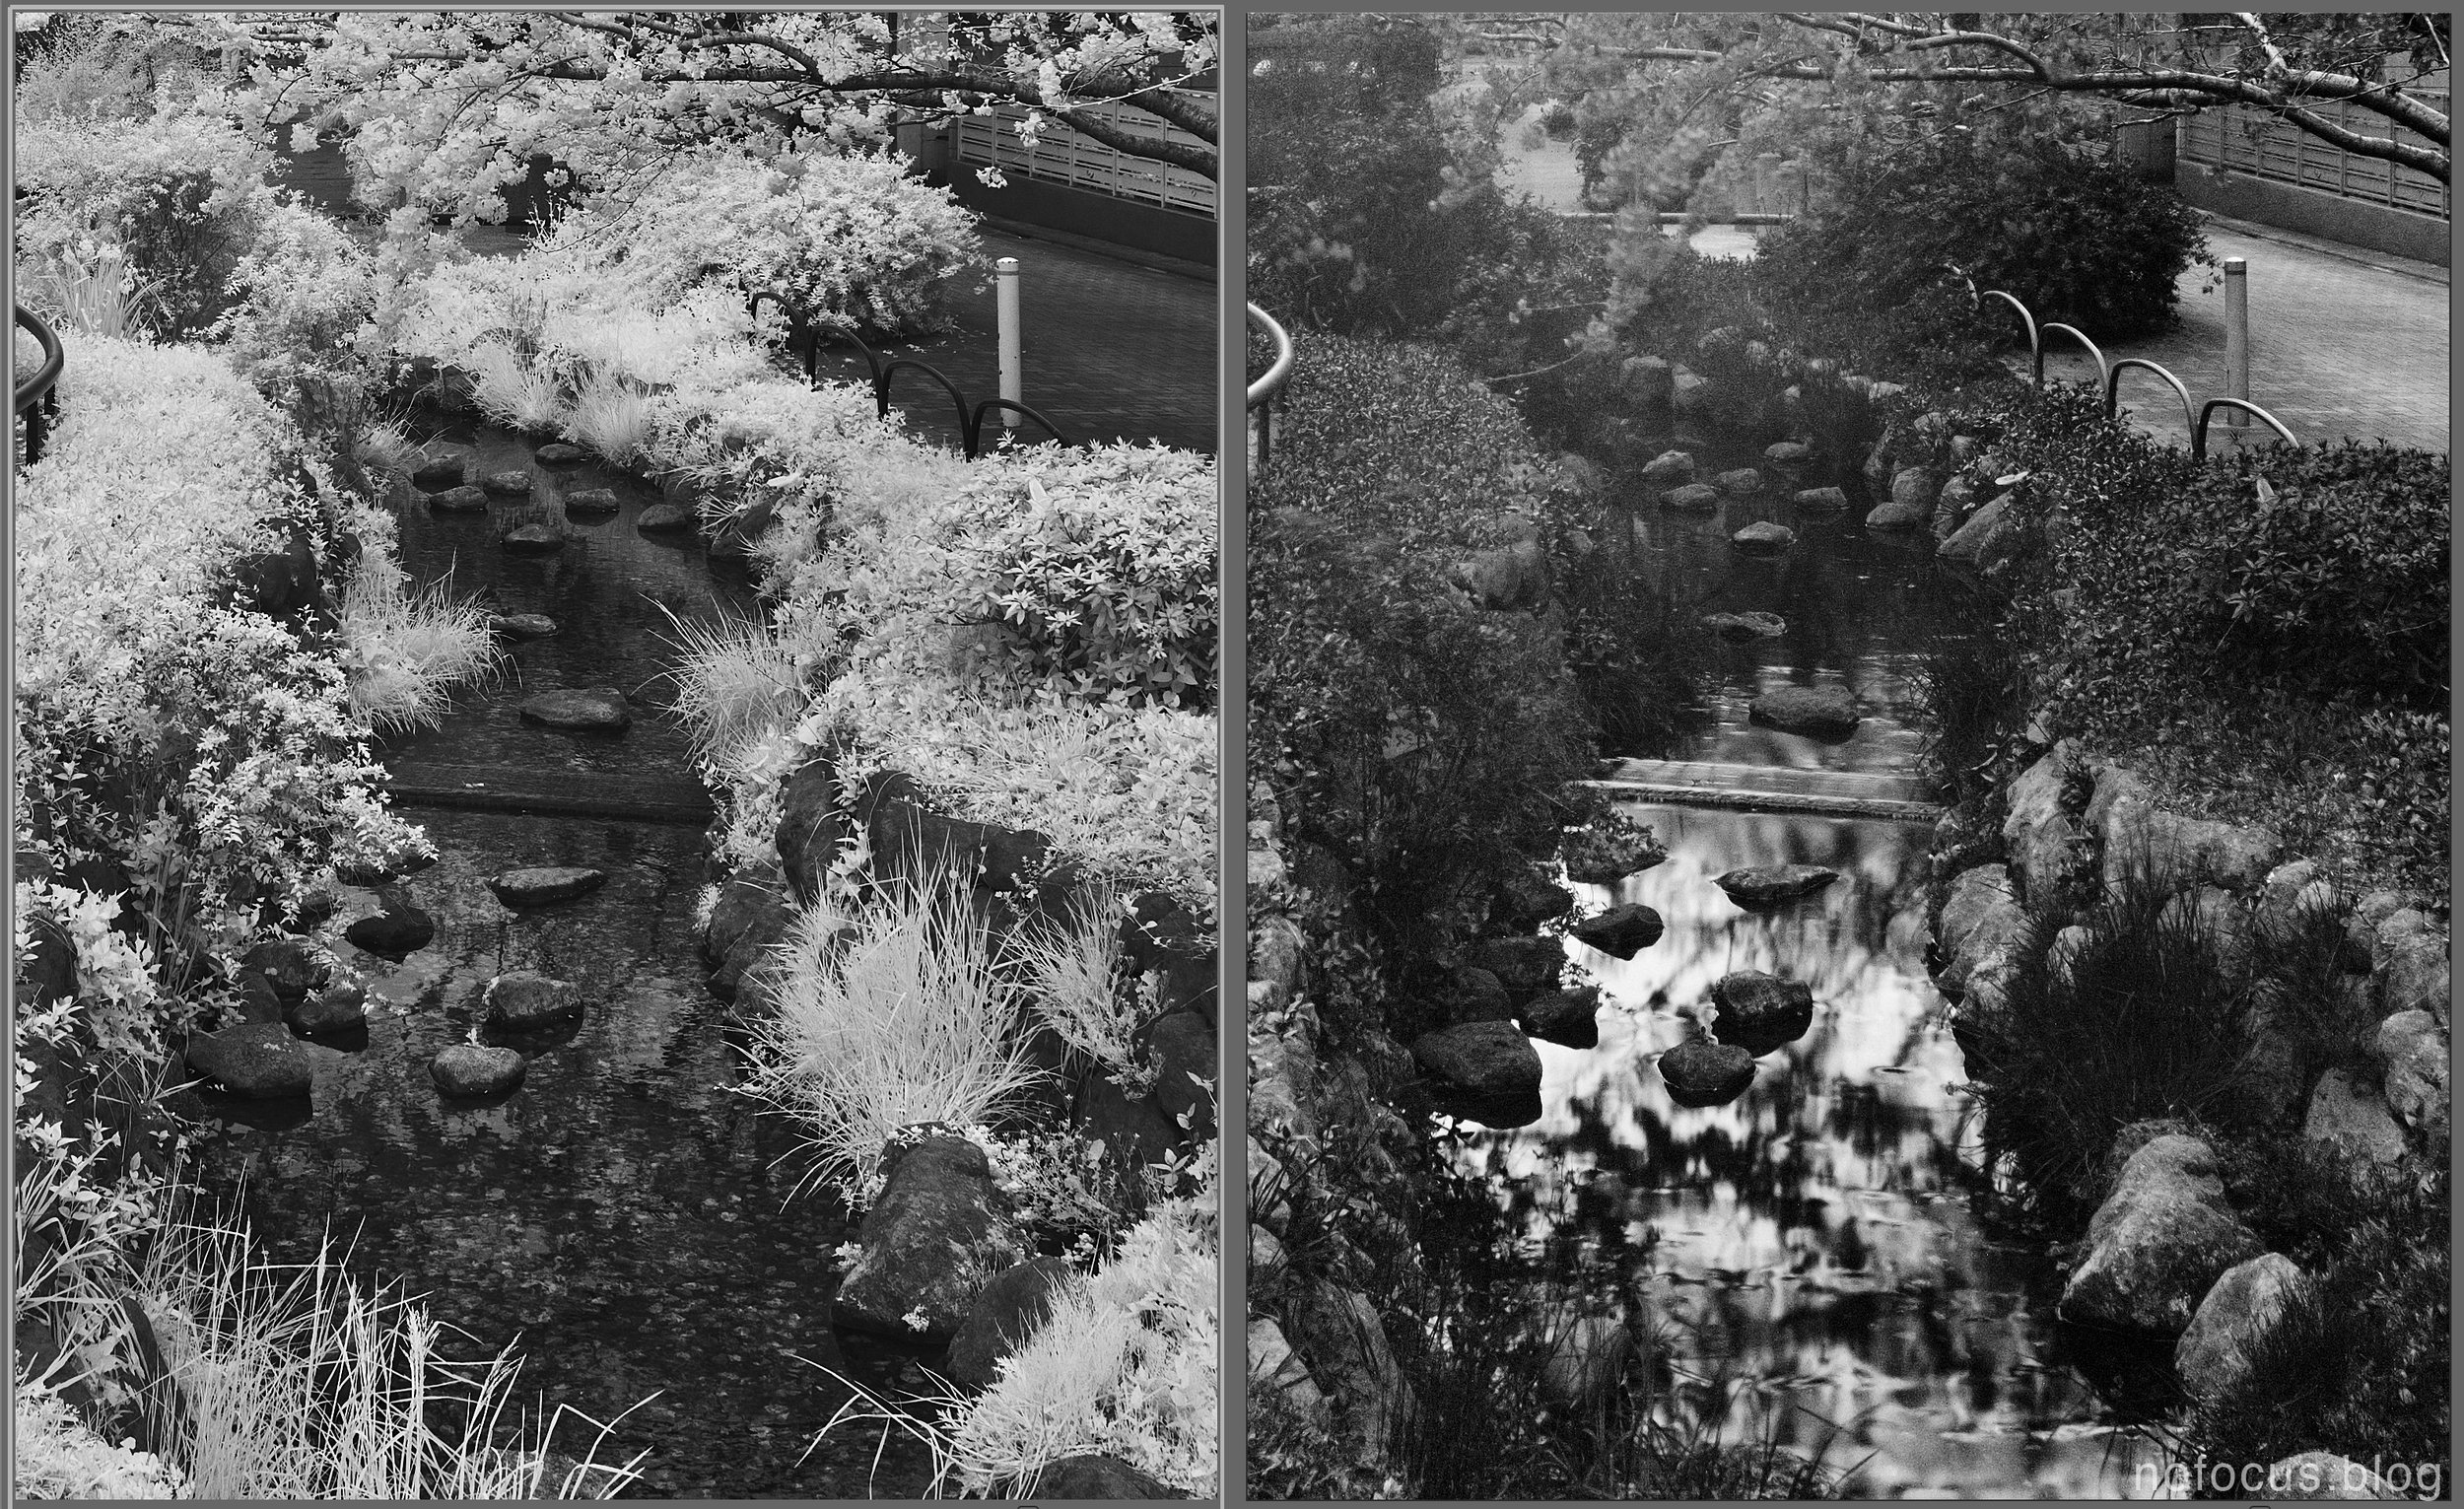
\includegraphics[width=.8\linewidth]{images/Infrared+photo+vs+Ultraviolet+photo.jpg}
		\hfill
	}	

	\caption{\label{fig:uv_ir_photo}
		Two views of the same scene: the left hand side
		shows intensity of a relatively narrow infrared band around 850 \unit{\nano\meter},
		while the right hand side shows ultraviolet light, 
		in the 345--380 \unit{\nano\meter} band. 
		Both bands are moderately beyond what is visible by humans}
	{\scriptsize\hfill
		Photograph by Tomas \url{https://www.nofocus.blog/}
	}
\end{figure}

As we have just seen, radiometric quantities can be used to measure brightness in 
terms of \emph{\gls{radiant power}} and its derived quantities.
However, if our image was generated using values proportional to this quantity,
we would obtain an image that will not correspond well to the subjective 
sense of brightness in the scene as experienced by a person looking at it. 
And it wouldn't look much like a black-and-white photograph either, not one made
with film stock a photographer would commonly use, or the black-and-white mode 
of a digital camera anyways.
There are two broad classes of reasons why this is the case: 
on the one side radiant power includes \emph{all} radiation
bands, and so this radiant power ``image'' would have information about all sorts 
of wavelengths that have little to do with vision. 
Let's imagine for a moment a semi-realistic scenario where we'd build a device 
capable of capturing energy of wavelengths in the millimeters (say radar waves 
or far infrared waves) all the way to maybe single nanometers\footnote{
	And for short wavelengths all sorts of
	problems appear, for example many materials such as flesh cease being opaque, or 
	scattering photons that much, a key capability for medical imaging} 
(which would be X-rays): it might be fun to try and imagine what pictures it would make.
This brings up many questions, for example: photons in longer wavelengths don't carry
all that much energy (one by one), so if we imagine that the number of photons arriving
is roughly even across wavelengths (say maybe in a range of $100:1$) we'd still need to make
up for the fact that one nanometer photon will be a million times brighter than one millimeter
photon, so it seems difficult to make useful pictures from such an incredibly wide dynamic range.
In fact, without going to these extremes, even bands quite near to the visible range look 
substantially different than they do in the visible, as you can see in~\cref{fig:uv_ir_photo}. 
The other class of reasons is that, even restricting ourselves to the visible range, 
our sensitivity to brightness exhibits a marked dependency on the wavelength 
(as you can see in a plot of the luminous efficiency 
function $V(\lambda)$, for example in~\cref{fig:illumspectra}).
When black and white film was originally developed this was a very carefully considered
affair, as you can see from~\cref{fig:orthopanphoto}.

\begin{figure}
	{
		\hfill
		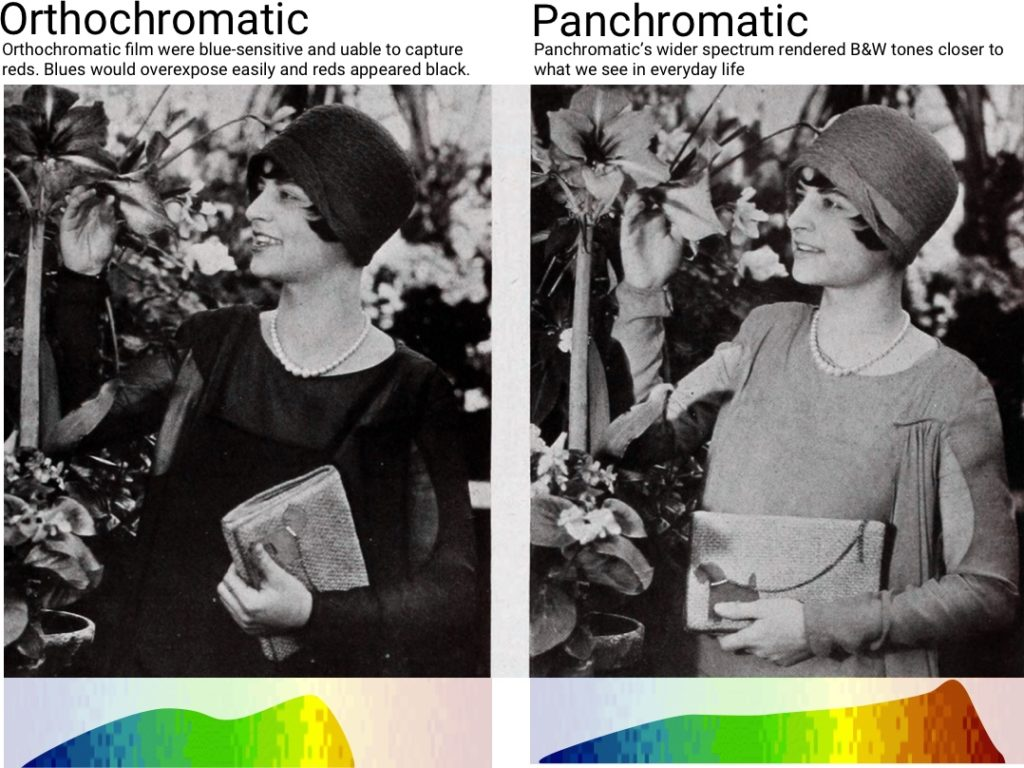
\includegraphics[width=.8\linewidth]{images/Orthochromatic-Panchromatic-film-1024x768-1.jpg}
		\hfill
	}	
	
	\caption{\label{fig:orthopanphoto}
		Reproduction of an old advertisement image, illustrating the difference between
		orthochromatic film, most sentitive to greens and blues, and panchromatic film,
		having a somewhat more even response across the visible spectrum. 
		Note that neither sensitivity curve is all that close to the luminous efficiency
		function $V(\lambda)$}
	{\scriptsize\hfill
		Photograph from \url{https://thedarkroom.com/orthochromatic-vs-panchromatic-film-a-photo-comparison/}
	}
\end{figure}

Because of how the human visual system is not equally sensitive to all wavelengths
of light, our eyes may well perceive light emanating or reflecting 
off two objects with different radiant intensity as having the same brightness, 
as a consequence of differences in the spectral distributions compensating 
away the difference in intensity. 
Conversely, \glspl{spectral distribution} carrying the same amount
of radiant power are likely to be perceived as having different brightness levels 
when they appear to have different colors.

It is therefore useful, and in a way \emph{necessary}, to reason about the power 
of light in two different ways, one dealing with energy levels as you would have in 
physics, called \textsl{radiometric}, and the other tuned or rebalanced, to account 
for the workings of human perception, called \textsl{photometric}\footnote{ 
The two approaches have historically used a great many units, 
until the \textsl{\gls{candela}} $[\unit\candela]$ was adopted as a base unit 
as part of Resolution 6 of the Tenth Conference on Weights and Measures
held in 1954~\cite[p. 163]{bipm:si.2019}, and then supplemented by derived units for
quantities \textsl{\gls{luminous flux}} $[\unit\lumen]$, 
\textsl{\gls{luminance}} $[\unit{\candela\per\square\meter}]$ 
and \textsl{\gls{illuminance}} $[\unit\lux]$ at the Eleventh Conference on Weights 
and Measures held in 1960.  
At this Eleventh conference the base units (which were six at the time) were first
given the name ``Syst\`eme International d’Unit\'es” and its abbreviation \glsname{si}.
Many more details around various historical and \gls{si} units are
described in~\cite{Meyer-Arendt:68}}. 
As discussed before, in this document we will use \gls{si} units and the harmonized 
vocabulary resulting from~\cite{iso:80000-7:2019,cie:s017.2020,iec:60050-845:2020}.

From the point of view of \textsl{\gls{radiometry}}, we saw how the \textsl{radiant power} 
of a source $S$ is measured in \textit{watts} $[\unit{\watt}]$ and is the total amount 
of energy per unit time emitted by $S$.
From the point of view of \textsl{\gls{photometry}}, there is a corresponding definition
of \textsl{luminous power} for our source $S$ (also called \textsl{luminous flux} as for the 
radiometry nomenclature) measured in \textit{lumens} $[\unit{\lumen}]$, and being the 
amount of energy per unit time weighted by the \textsl{photopic spectral luminous efficiency 
function} $V(\lambda)$. 
This function was designed to model the response of the human visual system as a function of 
wavelength $\lambda$\footnote{
	The photopic spectral luminous efficiency function $V(\lambda)$ is the result of a 
	series of experiments and tabulations first published by the \gls{CIE} in 1924 
	and then included as $\bar y(\lambda)$ in the color matching functions for 
	the \emph{standard 2 degree colorimetric observer}~\cite{smithguild1931}.}.

This means that two different light sources emitting the same luminous
power will appear as having about the same brightness even when having
different spectral distributions\footnote{This
	statement can only be true approximately, as the specific spectral response
	of different humans exhibits a certain amount of variation, even among normal 
	subjects.
	Also there are subjects having various different kinds of anomalies in their
	visual systems (called color vision deficiencies or color blindness), 
	for whom this statement ends up being even less accurate}.

Much like we've been using the subscript $\square_e$ to indicate radiant quantities such as
radiant power $\Phi_e$ or radiant intensity $I_e$, and the subscript $\square_{e,\lambda}$ to indicate
their spectral counterparts $\Phi_{e,\lambda}$ and $I_{e,\lambda}$, we will
indicate \emph{photometric} quantities with the subscript $\square_v$ for ``visual''.
Their definition follows one-to-one the corresponding radiometric quantity: for a
given radiometric spectral quantity $X_{e,\lambda}$ we can construct its
corresponding photometric quantity $X_v$ integrating like this
\begin{equation}
	X_v(\ldots) = K_{cd} \int X_{\lambda}(\ldots,\lambda)\; V(\lambda) \d\lambda.
\label{eqn:rad_to_photo}
\end{equation}
the corresponding names will also change, replacing ``(spectral) radiant'' with ``luminous''.
For example, given spectral radiant power $\Phi_{e,\lambda}(\lambda)$, the
corresponding luminous power $\Phi_v$ is
\begin{displaymath}
\Phi_v = K_{cd} \int \Phi_{e,\lambda}(\lambda)\; V(\lambda) \d\lambda \;[\unit\lumen]
\end{displaymath}

The scaling constant $K_{cd} = 683\;\unit{\lumen\per\watt}$, formally called \textsl{luminous efficacy of monochromatic radiation}, 
scales these ``reweighted watts'' to lumens and is currently one of the seven defining constants 
for the \gls{si}. 
As such it defines\footnote{
	The details of the current definition are in~\cite[p. 135]{bipm:si.2019}.
	The frequency of $\num{540}\;[\unit{\tera\hertz}]$ corresponds to a wavelength of 
	about $\num{555.016}\;[\unit{\nano\meter}]$ in \gls{standard air}, a wavelength in the 
	greens to which the eye of the standard observer is most sensitive.
	The radiant intensity of $1/683\;[\unit{\watt\per\steradian}]$ was chosen to make 
	the amount of $1\;[\unit\candela]$ about equal to the older unit
	\textit{standard candle}, which it superseded. 
	This definition has been updated several times from the original definition, 
	which had been established in 1933, based on the emission of a black body radiator
	at the freezing point of platinum (about $\num{2042}\;[\unit{\kelvin}]$). 
	This outdated definition is sometimes also found in 
	literature~\cite{Meyer-Arendt:68}.
} the base \gls{si} unit \textsl{candela} $[\unit{\candela}]$, 
as the amount of luminous intensity of a source of monochromatic radiation of frequency 
$\num{540}\;[\unit{\tera\hertz}]$ having a radiant intensity of $1/683\;[\unit{\watt\per\steradian}]$.

\ifomit

%This relates to the old definition of $K_m$, kept for archeological purposes

Using Eqn.~\eqref{eqn:rad_to_photo} and the Dirac delta distribution $\delta$, the
above definition can be written as
\begin{displaymath}
    1\,[\unit{\candela}] = 1\,\left[\unit{\lumen\per\steradian}\right]
    = K_m \int \frac{\delta(\lambda-555.016\unit{\nano\meter})}{683} \unit{\watt\per\steradian}\;V(\lambda) \d\lambda
    = K_m \cdot \frac{V(555.016\unit{\nano\meter})}{683}\,\left[\unit{\watt\per\steradian}\right],
\end{displaymath}
from which it follows that $K_{m} \approx 683.002 \;[\unit{\lumen\per\watt}]$. 
In practice, however, it is safe to use the value of 
$683\;[\unit{\lumen\per\watt}]$~\cite{cie:018.2019,wyszecki2000}.
\fi


\Cref{tab:radiophoto} lists summarized names, units and symbols of the radiometric quantities we've discussed,
as well as their spectral and photometric counterparts.

